\section*{2025年普通高等学校招生全国统一考试(新高考2卷)}
使用地区：海南、辽宁、重庆、吉林、黑龙江、贵州、广西、甘肃、云南、四川、陕西、山西、内蒙古、青海、宁夏\\
\parttitle{单选题}
\begin{example}{1}[2025][全国2卷][高三][高考][第1题]

样本数据2，8，14，16，20的平均数为\blankbox
\begin{choices}
\choice{$8$}
\choice{$9$}
\choice{$12$}
\choice{$18$}
\end{choices}


\begin{proof}
	\begin{answer}
		C
	\end{answer}
	\begin{solutions}
		平均数计算公式：$\bar{x}=\dfrac{2+8+14+16+20}{5}=12$，故选C。
	\end{solutions}
\end{proof}
\end{example}

\begin{example}{1}[2025][全国2卷][高三][高考][第2题]

若$z=1+\text{i}$，则$\dfrac{1}{z-1}=$\blankbox
\begin{choices}
\choice{$-\text{i}$}
\choice{$\text{i}$}
\choice{$-1$}
\choice{$1$}
\end{choices}


\kaodian{复数-复数代数形式的四则运算-复数的加减-复数加减法的代数运算}
\begin{proof}
	\begin{answer}
		A
	\end{answer}
	\begin{solutions}
		由$z=1+\text{i}$，得$z-1=\text{i}$，则$\dfrac{1}{z-1}=\dfrac{1}{\text{i}}=-\text{i}$，故选A。
	\end{solutions}
\end{proof}
\end{example}

\begin{example}{1}[2025][全国2卷][高三][高考][第3题]
设集合$A=\{-4,0,1,2,8\}$，$B=\{x\mid x^3=x\}$，则$A\cap B=$\blankbox
\begin{choices}
\choice{$\{0,1,2\}$}
\choice{$\{1,2,8\}$}
\choice{$\{2,8\}$}
\choice{$\{0,1\}$}
\end{choices}
\begin{proof}
	\begin{answer}
		D
	\end{answer}
	\begin{solutions}
		由$x^3=x$得$x(x^2-1)=0$，解得$x=-1,0,1$，即$B=\{-1,0,1\}$。
		又$A=\{-4,0,1,2,8\}$，故$A\cap B=\{0,1\}$，选D。
	\end{solutions}
\end{proof}
\end{example}

\begin{example}{1}[2025][全国2卷][高三][高考][第4题]
不等式$\dfrac{x-4}{x-1}\ge 2$的解集是\blankbox
\begin{choices}
\choice{$\{x\mid -2\le x\le 1\}$}
\choice{$\{x\mid x\le -2\}$}
\choice{$\{x\mid -2\le x<1\}$}
\choice{$\{x\mid x>1\}$}
\end{choices}

\end{example}

\begin{example}{1}[2025][全国2卷][高三][高考][第5题]
在$\triangle ABC$中，$AB=\sqrt{6}$，$BC=2$，$AC=1+\sqrt{3}$，则$A=$\blankbox
\begin{choices}
\choice{$45^\circ$}
\choice{$60^\circ$}
\choice{$120^\circ$}
\choice{$135^\circ$}
\end{choices}

\end{example}

\begin{example}{1}[2025][全国2卷][高三][高考][第6题]
设抛物线$C:y^2=2px(p>0)$的焦点为$F$，点$A$在$C$上，过$A$作$C$的准线的垂线，垂足为$B$，若$BF:y=-2x+2$，则$|AF|=$\blankbox
\begin{choices}
\choice{$3$}
\choice{$4$}
\choice{$5$}
\choice{$6$}
\end{choices}
\end{example}

\begin{example}{1}[2025][全国2卷][高三][高考][第7题]
记$S_n$等差数列$\{a_n\}$的前$n$项和，若$S_3=6$，$S_5=-5$，则$S_6=$\blankbox
\begin{choices}
\choice{$-20$}
\choice{$-15$}
\choice{$-10$}
\choice{$-5$}
\end{choices}
\end{example}

\begin{example}{1}[2025][全国2卷][高三][高考][第8题]
设$0<\theta<\pi$，若$\cos\dfrac{\theta}{2}=\dfrac{\sqrt{5}}{5}$，则$\sin\left(\theta-\dfrac{\pi}{4}\right)=$\blankbox
\begin{choices}
\choice{$\dfrac{\sqrt{2}}{10}$}
\choice{$\dfrac{\sqrt{2}}{5}$}
\choice{$\dfrac{3\sqrt{2}}{10}$}
\choice{$\dfrac{7\sqrt{2}}{10}$}
\end{choices}
\end{example}
\parttitle{多选题}
\begin{example}{2}[2025][全国2卷][高三][高考][第9题][多选]
记$S_n$等比数列$\{a_n\}$的前$n$项和，$\{a_n\}$的公比为$q$，若$q>0$，$S_3=7$，$a_3=1$，则\blankbox
\begin{choices}
\choice{$q=\dfrac{1}{2}$}
\choice{$a_5=\dfrac{1}{9}$}
\choice{$S_5=8$}
\choice{$a_n+S_n=8$}
\end{choices}
\end{example}

\begin{example}{2}[2025][全国2卷][高三][高考][第10题][多选]
已知$f(x)$是定义在$\mathbf{R}$上的奇函数，且当$x>0$时，$f(x)=(x^2-3)\text{e}^x+2$，则\blankbox
\begin{choices}
\choice{$f(0)=0$}
\choice{当$x<0$时，$f(x)=-(x^2-3)\text{e}^{-x}-2$}
\choice{$f(x)\ge 2$当且仅当$x\ge \sqrt{3}$}
\choice{$x=-1$是$f(x)$的极大值点}
\end{choices}
\end{example}

\begin{example}{2}[2025][全国2卷][高三][高考][第11题][多选]
双曲线$C:\dfrac{x^2}{a^2}-\dfrac{y^2}{b^2}=1(a>0,b>0)$的左右焦点分别为$F_1,F_2$．左右顶点分别为$A_1,A_2$，以$F_1F_2$为直径的圆与$C$的一条渐近线交于$M$，$N$两点，若$\angle MA_1N=\dfrac{5\pi}{6}$，则\blankbox
\begin{choices}
\choice{$\angle A_1MA_2=\dfrac{\pi}{6}$}
\choice{$|MA_1|=2|MA_2|$}
\choice{$C$离心率为$\sqrt{13}$}
\choice{当$a=\sqrt{2}$时，四边形$A_1MA_2N$的面积为$8\sqrt{3}$}
\end{choices}
\end{example}
\parttitle{填空题}
\begin{example}{3}[2025][全国2卷][高三][高考][第12题]
已知平面向量$\boldsymbol{a}=(x,1)$，$\boldsymbol{b}=(x-1,2x)$，若$\boldsymbol{a}\perp(\boldsymbol{a}-\boldsymbol{b})$，则$|\boldsymbol{a}|=$\blankline
\end{example}

\begin{example}{3}[2025][全国2卷][高三][高考][第13题]
若$x=2$是$f(x)=(x-1)(x-2)(x-a)$的极值点，则$f(0)=$\blankline
\end{example}

\begin{example}{3}[2025][全国2卷][高三][高考][第14题]
一个底面半径为$4\,\text{cm}$，高为$9\,\text{cm}$的封闭圆柱形容器（容器壁厚忽略不计）内有两个半径相等的铁球，则铁球半径的最大值为\blankline$\text{cm}$．
\end{example}
\parttitle{简答题}
\begin{example}{4}[2025][全国2卷][高三][高考][第15题]
已知$f(x)=\cos(2x+\varphi)(0\le \varphi<\pi)$，$f(0)=\dfrac{1}{2}$．
\begin{enumerate}
    \item 求$\varphi$；
    \item 设$g(x)=f(x)+f\left(x-\dfrac{\pi}{6}\right)$，求$g(x)$值域和单调区间．
\end{enumerate}
\end{example}

\begin{example}{4}[2025][全国2卷][高三][高考][第16题]
已知椭圆$C:\dfrac{x^2}{a^2}+\dfrac{y^2}{b^2}=1(a>b>0)$的离心率为$\dfrac{\sqrt{2}}{2}$，长轴长为$4$．
\begin{enumerate}
    \item 求$C$的方程；
    \item 过点$(0,-2)$的直线$l$与$C$交于$A$，$B$两点，$O$为坐标原点，若$\triangle OAB$面积为$\sqrt{2}$，求$|AB|$．
\end{enumerate}
\end{example}

\begin{example}{4}[2025][全国2卷][高三][高考][第17题]
如图，在四边形$ABCD$中，$AB\parallel CD$，$\angle DAB=90^\circ$，$F$为$CD$中点，$E$在$AB$上，$EF\parallel AD$，$AB=3AD$，$CD=2AD$．将四边形$EFDA$沿$EF$翻折至四边形$EFD'A'$，使得面$EFD'A'$与面$EFCB$所成的二面角为$60^\circ$．
\begin{enumerate}
    \item 证明：$A'B\parallel$平面$CD'F$；
    \item 求平面$BCD'$与面$EFD'A'$所成二面角的正弦值．
\end{enumerate}

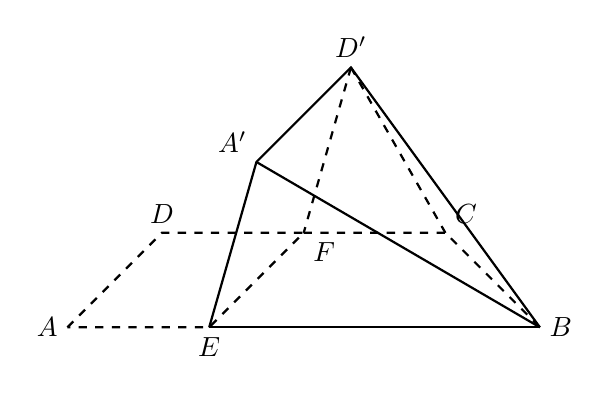
\begin{tikzpicture}[scale=1.5, >=latex]
	% 1. 定义底面固定坐标（不变）
	\coordinate (A) at (-1.5,-0.5);
	\coordinate (D) at (-0.7,0.3);
	\coordinate (E) at (-0.3,-0.5);
	\coordinate (F) at (0.5,0.3);
	
	% 右侧固定点（不变）
	\coordinate (B) at (2.5,-0.5);
	\coordinate (C) at (1.7,0.3);
	
	% 核心修改：调整 A'、D' 坐标，模拟 120° 空间翻折角
	\coordinate (A') at (0.1, 0.9);   % 120°翻折后 A 的投影
	\coordinate (D') at (0.9, 1.7);   % 120°翻折后 D 的投影
	
	% 2. 绘制不可见线与原平面残留（虚线段）
	\draw[dashed, thick] (A) -- (D) -- (F) -- (E) -- (A);
	\draw[dashed, thick] (F) -- (C) -- (B);
	\draw[dashed, thick] (D') -- (F);
	\draw[dashed, thick] (D') -- (C);
	
	% 3. 绘制可见线（实线段）
	\draw[thick] (E) -- (B);
	\draw[thick] (E) -- (A') -- (D') -- (B);
	\draw[thick] (A') -- (B);
	
	% 4. 顶点标注
	\node[left] at (A) {$A$};
	\node[above] at (D) {$D$};
	\node[below] at (E) {$E$};
	\node[below right] at (F) {$F$};
	\node[right] at (B) {$B$};
	\node[above right] at (C) {$C$};
	\node[above left] at (A') {$A'$};
	\node[above] at (D') {$D'$};
	
\end{tikzpicture}
\end{example}

\begin{example}{4}[2025][全国2卷][高三][高考][第18题]
已知函数$f(x)=\ln(1+x)-x+\dfrac{1}{2}x^2-kx^3$，其中$0<k<\dfrac{1}{3}$．
\begin{enumerate}
    \item 证明：$f(x)$在$(0,+\infty)$存在唯一极值点和唯一零点；
    \item 设$x_1,x_2$为$f(x)$在$(0,+\infty)$的极值点和零点．
    \begin{enumerate}
        \item 设函数$g(t)=f(x_1+t)-f(x_1-t)$，证明：$g(t)$在$(0,x_1)$单调递减；
        \item 比较$2x_1$与$x_2$的大小，并证明．
    \end{enumerate}
\end{enumerate}
\end{example}

\begin{example}{4}[2025][全国2卷][高三][高考][第19题]
甲、乙两人进行乒乓球练习，每个球胜者得1分，负者得0分．设每个球甲胜概率为$p\left(\dfrac{1}{2}<p<1\right)$，乙胜概率为$q$，$p+q=1$，且各球的胜负相互独立．对正整数$k\ge 2$，记$P_k$为打完$k$个球后甲比乙至少多得2分的概率，$q_k$为打完$k$个球后乙比甲至少多得2分的概率．
\begin{enumerate}
    \item 求$P_3$，$P_4$（用$p$表示）；
    \item 若$\dfrac{P_4-P_3}{q_4-q_3}=4$，求$p$；
    \item 证明：当$m\in \mathbf{N}^*$时，$P_{2m+1}-q_{2m+1}<P_{2m}-q_{2m}<P_{2m+2}-q_{2m+2}$．
\end{enumerate}
\end{example}